\chapter{Introduction}

\section{Motivation}

In the past five decades, the world has undergone a demographic transformation
of unprecedented scale and pace. The global urban population has grown from fewer
than one billion people in 1960 to more than four billion today, a trajectory
projected to intensify throughout the remainder of the twenty-first century as
populations across Asia, Africa, and Latin America continue migrating toward
metropolitan centers in pursuit of economic opportunity, social mobility, and
access to public services.\footnote{UN-Habitat (2020). \textit{World Cities
Report 2020: The Value of Sustainable Urbanization.}
\url{https://unhabitat.org/world-cities-report-2020-the-value-of-sustainable-urbanization}}
This concentration of human activity within urban boundaries has made cities
simultaneously the principal engines of global economic productivity and the
foremost sites of environmental pressure: they account for approximately 70
percent of total energy consumption, generate a commensurate share of greenhouse
gas emissions, and place relentless demand on water, transportation, and
sanitation infrastructure. The capacity to accurately monitor, quantify, and
interpret the spatial dynamics of urban growth has therefore emerged as a
foundational requirement for sustainable development planning, disaster risk
reduction, and evidence-based governance at all scales of public administration.

Lima Metropolitan Area exemplifies with singular clarity the tensions
characterizing urban expansion in the Global South. Home to more than ten million
inhabitants concentrated in one of the driest coastal desert environments on
Earth and situated along one of the world's most seismically active subduction
zones, Lima's built fabric has grown through a dual process of horizontal
extension and vertical intensification.\footnote{Instituto Nacional de
Estadística e Informática (INEI), Censo Nacional de Población 2017.
\url{https://censo2017.inei.gob.pe/resultados-definitivos-de-los-censos-nacionales-2017/}}
Horizontal expansion refers to the occupation of previously undeveloped land at
the urban periphery: hillside settlements constructed with no formal engineering
oversight, informal subdivisions extending across desert flatlands, and the
gradual absorption of adjacent agricultural and ecological zones into the
consolidated metropolitan area.\footnote{Water-Sensitive Urban Plan for Lima
Metropolitan Area (Peru) Based on Changes in the Urban Landscape from 1990 to
2021. doi: \url{https://doi.org/10.3390/land11122261}}
Vertical densification, by contrast, refers to the progressive addition of
storeys to existing building stock---a phenomenon documented in Lima's
consolidated residential districts, where rising land values and in-situ
population pressure compel owners to maximize floor area within existing
footprints.\footnote{Confederación Nacional de Instituciones Empresariales
Privadas (2013, December 13). Residential buildings in Lima gained two floors
in height since 2011. CONFIEP.
\url{https://www.confiep.org.pe/noticias/edificios-de-viviendas-en-lima-ganaron-dos-pisos-en-altura-desde-el-2011/}}
Both modalities impose distinct demands on infrastructure networks, seismic load
calculations, and public utility capacity, yet they differ fundamentally in their
spectral and geometric signatures in satellite imagery, making their automated
discrimination a genuinely non-trivial remote sensing challenge. National census
data, updated only once per decade, cannot capture the velocity of contemporary
change, and municipal cartographic records frequently lag behind de facto
construction activity by years, leaving planning agencies without timely spatial
information at the resolution needed for effective intervention.

\begin{figure}[h!]
    \centering
    \begin{subfigure}[b]{0.45\textwidth}
        \centering
        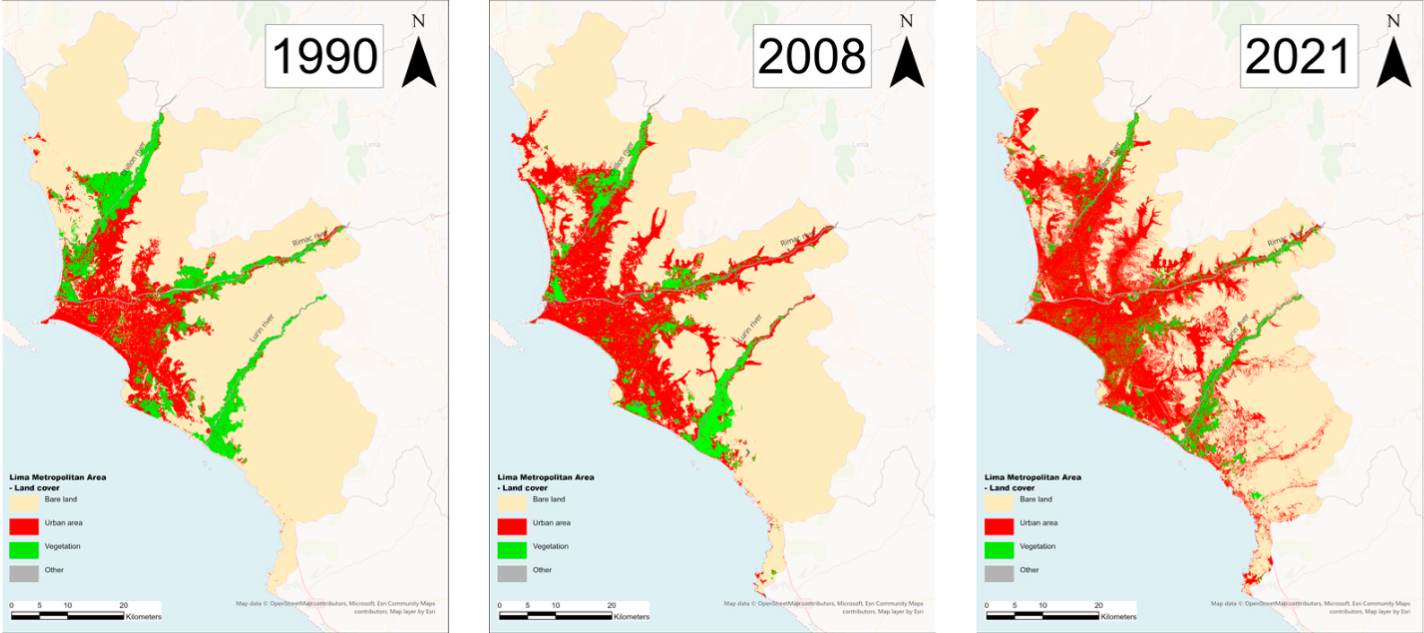
\includegraphics[height=6cm]{graficos/horizontal.png}
        \caption{Urban horizontal expansion: progressive occupation of peripheral
        land by new residential and commercial settlements.}
        \label{fig:horizontal}
    \end{subfigure}
    \hfill
    \begin{subfigure}[b]{0.45\textwidth}
        \centering
        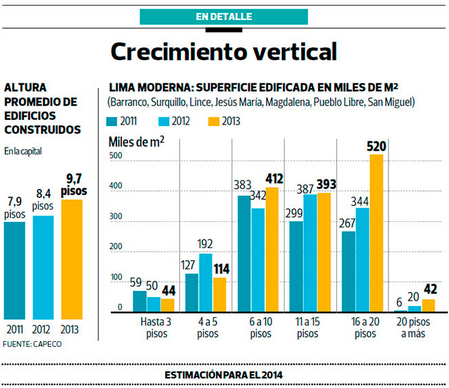
\includegraphics[height=6cm]{graficos/vertical.png}
        \caption{Urban vertical densification: addition of storeys to existing
        building stock within consolidated urban zones.}
        \label{fig:vertical}
    \end{subfigure}
    \caption{The two primary modalities of urban growth observable in Lima
    Metropolitan Area. An automated change detection system must discriminate
    between these structurally distinct patterns to provide decision-relevant
    intelligence for urban planning and infrastructure management.}
    \label{fig:comparison_growth}
\end{figure}

Very high-resolution (VHR) satellite imagery offers the most promising
technological pathway for addressing this monitoring gap at scale. Contemporary
Earth observation missions, including the Peruvian satellite PeruSAT-1, are
capable of acquiring panchromatic imagery at 0.70 meters per pixel and
multispectral imagery at 2.80 meters per pixel, thereby resolving individual
building footprints, rooftop configurations, and construction material
characteristics across large geographic extents within a single orbital pass.
By comparing co-registered image pairs acquired at different temporal epochs,
automated building change detection (BCD) algorithms can identify which
structures have appeared, disappeared, expanded, or undergone material
modification between acquisition dates, a capability of direct operational
value---as reviewed by \cite{Cheng2021DeepLab}---for urban planning, informal
settlement monitoring, post-disaster damage assessment, and infrastructure
auditing. The central
methodological challenge, however, is that the volumes of imagery generated by
modern satellite constellations far exceed the annotation and manual analysis
capacity of expert practitioners, and the heterogeneous radiometric conditions,
geometric misregistration, and seasonal spectral variation inherent in
multitemporal archives severely complicate straightforward image-differencing
approaches. Deep learning has therefore emerged, as documented
by \cite{Sirko2023TeachStudentSentinel2}, as the only viable paradigm for
scalable, robust BCD at city or regional scale.

\begin{figure}[htbp]
    \centering
    \begin{subfigure}[b]{0.48\linewidth}
        \centering
        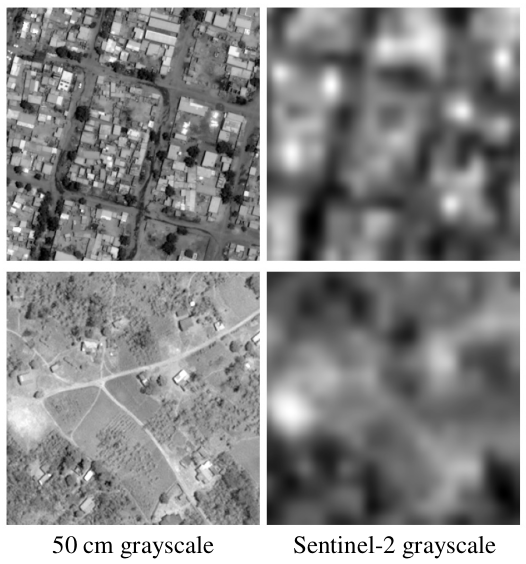
\includegraphics[width=\linewidth, height=6.5cm]{graficos/VHR-sentinel2.png}
        \caption{Comparison of VHR imagery against medium-resolution Sentinel-2 (10~m/pixel): individual buildings cannot be resolved at medium resolution.}
    \end{subfigure}
    \hfill
    \begin{subfigure}[b]{0.48\linewidth}
        \centering
        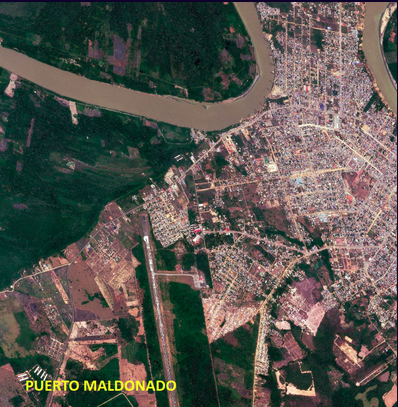
\includegraphics[width=\linewidth, height=6.4cm]{graficos/PeruSAT1.png}
        \caption{PeruSAT-1 panchromatic imagery at 0.70~m/pixel, sufficient to delineate individual building footprints and rooftop configurations.}
    \end{subfigure}
    \caption{Spatial resolution comparison between satellite imaging systems. VHR missions such as PeruSAT-1 are essential for building-level change detection, whereas medium-resolution sensors provide broad coverage without the spatial detail required to resolve structural modifications in the built environment.}
    \label{fig:resolution_comparison}
\end{figure}

The past decade has witnessed a decisive paradigm shift in remote sensing change
detection, driven by the exceptional representational capacity of deep learning
architectures. Following the success of fully convolutional networks and
encoder-decoder designs adapted for semantic segmentation, the introduction of
attention mechanisms and Vision Transformer (ViT) backbones
\cite{Vaswani2017Attention, Dosovitskiy2021ViT} opened a new frontier for
modeling non-local spatial and temporal dependencies across entire image regions.
Within the BCD domain, architectures such as the Binary change detection with
Image Transformers (BIT) \cite{Chen2022BIT}, SNUNet-CD \cite{Fang2021SNUNetCD},
and ChangeFormer \cite{Bandara2022ChangeFormer} demonstrated that globally
context-aware, hierarchical Siamese encoders equipped with multi-head
self-attention substantially outperform locally-receptive convolutional
predecessors on challenging urban datasets, with ChangeFormer
\cite{Bandara2022ChangeFormer} achieving state-of-the-art accuracy on the
LEVIR-CD benchmark \cite{Zheng2020LEVIR}. These advances confirmed a
generalized principle: accurate discrimination of building-scale structural
changes requires simultaneous sensitivity to fine-grained local texture
differences and broad spatial context, as independently demonstrated
\cite{Zheng2022HFANet, Teng2023SwinCD}, capable of disambiguating true
construction events from radiometric artifacts, illumination variations, and
seasonal phenological effects.

The representational advantages of Transformer-based BCD, however, carry a
computational cost that constitutes a critical accessibility barrier. Standard
multi-head self-attention scales quadratically in both time and memory with
respect to the number of input tokens---a regime that becomes acutely limiting
in VHR remote sensing, where even moderate patch sizes generate hundreds of
spatial embeddings, and bi-temporal pipelines further amplify this burden by
processing pre-event and post-event images through shared encoder streams.
Researchers operating outside high-performance computing environments---a
condition representative of the vast majority of academic and public-sector
institutions in Latin America and the Global South---find that this memory
footprint constrains feasible batch sizes, effective training resolutions, and
iteration speed to a degree that impedes systematic model development and
comparative experimentation. Rank-Augmented Linear Attention (RALA), as
formalized by \cite{Fan2025RALA}, constitutes a principled architectural
response to this constraint: by reformulating the key-value aggregation step as
a rank-augmented weighted buffer, it reduces attention-related peak GPU memory
consumption by approximately 22 percent and increases the maximum feasible
training batch size by up to 50 percent at standard processing resolutions---
efficiency gains that meaningfully democratize access to Transformer-based BCD
for research groups operating under constrained hardware budgets. Integrating
RALA into the encoder of ChangeFormer therefore offers the opportunity to extend
state-of-the-art change detection capacity to resource-limited environments,
including those engaged in VHR urban monitoring of Peruvian cities with
PeruSAT-1 imagery.


\section{Problem}

The central architectural bottleneck addressed in this thesis arises from the
computational properties of standard multi-head self-attention (MHSA) in
Transformer-based change detection networks. In MHSA, each token in the input
sequence attends to all other tokens by computing pairwise similarity scores,
forming a dense interaction matrix whose size, as established by
\cite{Vaswani2017Attention}, grows as the square of the sequence length.
In natural image classification tasks, where
input sequences are relatively short and a single global representation suffices,
this quadratic regime remains tractable. In bi-temporal VHR building change
detection, two compounding factors transform this scaling behavior into a decisive
practical constraint: the spatial resolution of VHR inputs generates long token
sequences at each encoder level, and the inherently bi-temporal nature of the
task effectively doubles the token count within each forward pass by processing
pre-event and post-event image patches together. The result is a memory
consumption profile that grows prohibitively as either input resolution or batch
size increases---a property that is particularly severe in hierarchical Siamese
architectures such as ChangeFormer \cite{Bandara2022ChangeFormer}, where MHSA
operates across multiple scales simultaneously and token counts at finer encoder
stages remain substantial.

The practical ramifications of this quadratic regime manifest directly in the
experimental constraints facing researchers without access to high-memory GPU
clusters. Under a 40~GB VRAM budget---representative of modern academic computing
environments---a standard ChangeFormer model operating at $256 \times 256$ patch
resolution supports a maximum batch size of 32 images per training iteration;
scaling the patch resolution to $512 \times 512$ reduces this to 8 images, and
operating at the native $1024 \times 1024$ resolution of the LEVIR-CD dataset
reduces the feasible batch size to 2---a regime in which gradient estimation
becomes noisy, convergence becomes unreliable, and the statistical diversity of
training samples per update is severely diminished. These constraints are not
merely inconveniences of scale: small effective batch sizes impair the
representativeness of gradient updates, slow the learning trajectory on
heterogeneous datasets, and make it impractical to evaluate the effect of input
resolution on detection accuracy---a parameter of particular relevance for
PeruSAT-1 applications, where the 0.70~m per pixel panchromatic resolution
demands high-resolution processing to resolve fine-grained structural changes
such as rooftop modifications or single-storey additions. The combinatorial
effect is a systematic reduction in research throughput and model exploration
capacity for institutions operating without large-scale GPU infrastructure.

An apparently natural remedy is to substitute the quadratic softmax attention
kernel with a linear feature map, reducing the attention complexity from
quadratic to linear in the sequence length. This family of efficient attention
mechanisms has attracted substantial theoretical and empirical interest in the
broader machine learning community. However, a critical failure mode has been
formally identified for linear attention in dense prediction settings: the
intermediate key-value aggregation buffer of linear attention tends toward
rank collapse, a degeneration in which the aggregated sequence representation
occupies a low-dimensional subspace that discards the spatial diversity essential
for pixel-accurate segmentation and change localization. Earlier efficient
attention methods demonstrated measurable accuracy degradation on dense vision
benchmarks precisely for this reason, undermining their practical utility for
change detection applications where precise boundary delineation is required.
RALA \cite{Fan2025RALA} directly addresses rank collapse through a learned,
token-wise reweighting of key-value contributions augmented by a channel-wise
output modulation step that restores feature diversity without reintroducing
quadratic cost. The central research hypothesis motivating this thesis is
therefore the following: when the rank-augmented linear attention mechanism of
RALA is systematically substituted for the standard MHSA modules within the
hierarchical encoder of ChangeFormer, can the resulting model maintain
segmentation accuracy comparable to the quadratic baseline across diverse
building change detection benchmarks spanning multiple acquisition geometries
and scene complexities---while simultaneously delivering meaningful reductions
in GPU memory consumption and enabling larger, more stable training
configurations?


\section{Goals}

The primary objective of this thesis is to design, implement, and rigorously
validate \textbf{RALA-ChangeFormer}, a computationally efficient hierarchical
Siamese Transformer architecture for multi-temporal building change detection
from VHR satellite imagery. The proposed architecture pursues the replacement of
standard quadratic self-attention within the encoder stages of ChangeFormer with
rank-augmented linear attention \cite{Fan2025RALA}, with the dual ambition of
reducing attention-related computational cost from quadratic to near-linear
complexity while preserving the segmentation accuracy of the baseline model
across diverse urban environments and acquisition conditions. This primary
objective is motivated not only by the theoretical interest of studying
efficiency-accuracy trade-offs in bi-temporal Transformer architectures, but
also by the applied imperative of extending state-of-the-art change detection
capabilities to research and operational contexts where access to large-memory
GPU infrastructure cannot be assumed---including Peruvian institutions, such as
the Urban Data Analysis subgroup within GINIA at UTEC, engaged in monitoring
PeruSAT-1 imagery of Lima Metropolitan Area and other rapidly growing South
American cities.

The realization of this primary objective is pursued through a coherent sequence
of specific operational goals. The first concerns the rigorous architectural
design and software implementation of the RALA-ChangeFormer encoder, requiring
the adaptation of the rank-augmentation mechanism to the multi-scale, hierarchical
token structure of ChangeFormer \cite{Bandara2022ChangeFormer} and the
verification of tensor-dimensional compatibility, numerical stability, and
accurate computational profiling across all encoder stages. The second goal is
a comprehensive efficiency analysis that quantifies, under controlled experimental
conditions, the reductions in floating-point operations (FLOPs), peak GPU memory
consumption, maximum feasible batch size, and per-epoch training throughput
achieved by RALA relative to the quadratic baseline---providing empirical grounding
for the argument that efficient attention mechanisms are a meaningful tool for
broadening access to advanced BCD research. The third, and most extensive, goal
is the systematic cross-domain evaluation of RALA-ChangeFormer across six
geographically and methodologically diverse benchmarks: the LEVIR-CD and
DSIFN-CD datasets that constitute the foundational experimental suite, together
with four extended datasets---WHU-CD, LEVIR-CD+, SYSU-CD, and S2Looking---
spanning a range of acquisition geometries from nadir-view centimetre-resolution
aerial imagery to oblique side-looking satellite acquisitions, annotation quality
levels from precisely delineated building footprints to multi-class surface
change labels, and scene heterogeneity conditions from homogeneous planned urban
developments to complex informal settlement environments. This extended
experimental program is designed not merely to assess whether RALA-ChangeFormer
achieves performance parity with the baseline under standard benchmark conditions,
but to identify the generalization boundaries of rank-augmented linear attention:
the acquisition characteristics that preserve the efficiency advantage without
accuracy sacrifice, and the failure modes that motivate further architectural
development.

The remainder of this document is organized to build progressively from
conceptual foundations toward full experimental validation.
Chapter~\ref{chap:background} establishes the theoretical prerequisites required
to understand the proposed method, covering the principles of satellite imagery
and spatial resolution, the formal definition of the bi-temporal building change
detection problem, the mathematical structure of multi-head self-attention and
its quadratic complexity, the rank-augmented linear attention formulation
underpinning RALA, and the evaluation metrics employed throughout this work.
Chapter~\ref{chap:related_work} situates the contribution within the existing
literature by reviewing supervised, semi-supervised, and self-supervised learning
strategies for BCD, the progression from convolutional Siamese networks to
hierarchical Transformer architectures, and the landscape of efficient attention
mechanisms and their known limitations in dense prediction settings.
Chapter~\ref{chap:method} details the complete RALA-ChangeFormer pipeline,
including the preprocessing stages applied to bi-temporal image pairs, the
precise integration of rank-augmented attention into each encoder block, the
hybrid loss function, and the post-processing localization procedure that
converts model outputs into interpretable binary change masks.
Chapter~\ref{chap:experiments} presents the full experimental evaluation,
encompassing quantitative accuracy and efficiency comparisons across all six
benchmarks, qualitative analysis of predicted change masks and attention
distributions, training dynamics under each acquisition condition, and a
substantive discussion of the performance gradient observed across datasets of
varying geometric and spectral complexity. Finally,
Chapter~\ref{chap:conclusiones} synthesizes the principal findings, enumerates
the current limitations of the proposed approach, and outlines future research
directions including geometric alignment for oblique-view imagery, dynamic rank
adaptation strategies, and the construction of dedicated building change
detection benchmarks for the heterogeneous urban environments of the Global South.
